% Uncomment this line for on-screen presentation
\documentclass[xcolor={dvipsnames}]{beamer}\usepackage{etoolbox}\newtoggle{printable}\togglefalse{printable}

% Uncomment this line for printable slides (disable animations and don't waste ink)
%\documentclass[handout, xcolor={dvipsnames}]{beamer}\usepackage{etoolbox}\newtoggle{printable}\toggletrue{printable}

% Adjust these for the path of the theme and its graphics, relative to this file
%\usepackage{beamerthemeFalmouthGamesAcademy}
\usepackage{../../beamerthemeFalmouthGamesAcademy}
\graphicspath{ {../../} }

% Default language for code listings
\lstset{language=C++,
		morekeywords={each,in}
}

\begin{document}
\title{Introduction to HCI for Games}   
\subtitle{COMP140: Creative Computing Hacking}

\frame{\titlepage} 

\begin{frame}{Course Objectives}
	The following three lectures have been designed to provide an introduction to and provide support for your next creative computing project:
	
	\begin{itemize}
		\item \textbf{Design and Prototype} a novel game controller.
		\item \textbf{Evaluate} the role of your controller in one of the games being developed by students on the BA Digital Games course; \textbf{or}
                      the game you developed in COMP130 last semester.
	\end{itemize}
\end{frame}

\begin{frame}{Important Notice}
	\begin{columns}[onlytextwidth]
		\begin{column}{0.45\textwidth}
			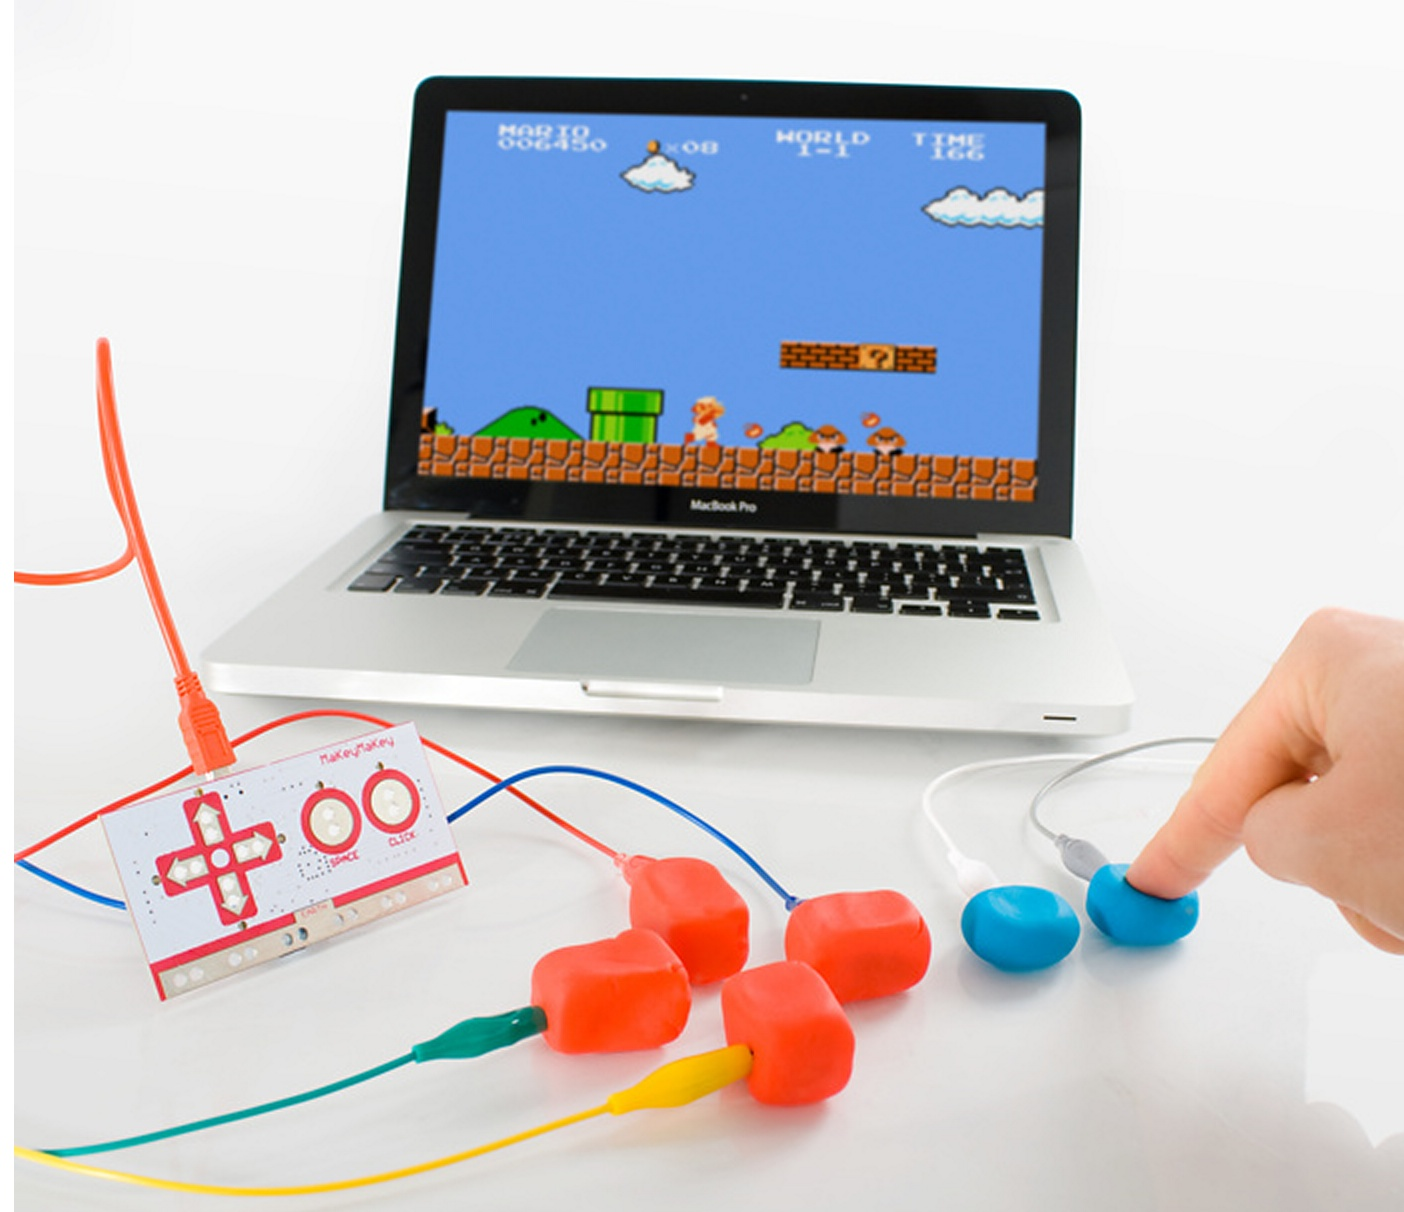
\includegraphics[height=22ex]{MakeyMakey.jpg}
		\end{column}
		\begin{column}{0.45\textwidth}
			Remember to bring your \textit{Makey Makey} kit and associated materials to these lectures for practical 
			support toward the end of each of these sessions.
		\end{column}
	\end{columns}
\end{frame}

\part{HCI and Interactive Systems}
\frame{\partpage}

\begin{frame}{Learning Outcomes}
	In this section you will learn how to...
	
	\begin{itemize}
		\item \textbf{Describe} the increasing role of interactive systems in computing
		\item \textbf{Describe} the role of HCI in system design
		\item \textbf{Demonstrate} an awareness of the HCI viewpoint which places the player at the centre of design
		\item \textbf{Describe} HCI's component disciplines and the contributions they make to it
	\end{itemize}
\end{frame}

\begin{frame}{Further Reading}
	\begin{itemize}
		\item Dix, A., Finlay, J., Abowd, G., Beale, R. (1998) \textit{Human-Computer Interaction}. 2nd Edition. Prentice Hall.
		\item Newman, W.M. and Lamming, M.G. (1994) \textit{Interactive System Design}. Addison-Wesley.
		\item Preece, J., Rogers, Y., Sharp, H., Benyon, D., Holland, S., and Carey, T. (1994) \textit{Human-Computer Interaction}. Addison-Wesley.
	\end{itemize}
\end{frame}

\begin{frame}[fragile]{Socrative \texttt{JBYPC3BBY}}
    \textbf{What} is Human-Computer Interaction?
\end{frame}

\begin{frame}[fragile]{Socrative \texttt{JBYPC3BBY}}
    \textbf{Why} is HCI relevant to games?
\end{frame}

\begin{frame}{HCI and Interactive Systems}
	It is...
	\begin{itemize}
		\item An academic discipline: studying people interacting with technology
		\item A design discipline: designing interventions for systems involving people and technology
	\end{itemize}
\end{frame}

\begin{frame}{HCI and Interactive Systems}
	It is important to distinguish between \textbf{the subject of human-computer interaction} and the notion of
	\textbf{a human computer interface}:
	
	\begin{itemize}
		\item Human-computer action is ``the disciplines concerned with the design, evaluation, 
		and implementation of interactive computer systems for human use and the study of major phenomena
		surrounding them'' (Dix, 1998, xi). It involves understanding, analysing, and implementing computer
		systems for human use.
	\end{itemize}
\end{frame}

\begin{frame}{HCI and Interactive Systems}
	It is important to distinguish between \textbf{the subject of human-computer interaction} and the notion of
	\textbf{a human computer interface}:
	
	\begin{itemize}
		\item The human-computer interface involves those aspects of a system that users interact with. That is,
		the \textit{zone of interaction}. It is the part of the computer system that provided access to a computers
		internal resources. This is a technology, rather than a discipline.
	\end{itemize}
\end{frame}

\begin{frame}{HCI and Interactive Systems}
	In the early era of computing, the `ease of use' of interfaces was given little attention:
	
	\begin{itemize}
		\item Restricted access
		\item Specialist users
		\item Very specific use-cases for computers
	\end{itemize}
\end{frame}

\begin{frame}{HCI and Interactive Systems}
	Now that technology has matured enough for games to evolve into a mass-market phenomena, it is now a goal for
	computer systems to be made more accessible to a wider range of users for a greater variety of interaction styles. 
	
	\begin{itemize}
		\item This is only possible by designing for the needs of such players
		\item Expecting players to adapt is inappropriate, they simply won't buy your games
		\item Incompetence-inducing controls are linked to aggression (Przybylski \textit{et al}, 2014)
	\end{itemize}
\end{frame}

\begin{frame}{HCI and Interactive Systems}
	For interactive systems such as games this has come to mean designing the user interface. 
	
	\begin{itemize}
		\item The part of the system which the user is in immediate contact
		\item This includes input and output devices.
		\item Estimates suggest anything up to 80\% of the code supports the interface (Perry, 2006)
		\item A great deal of development time and effort is required working with people to achieve high usability --- 
		very different to the `being a basement code monkey' myth
	\end{itemize}
\end{frame}

\begin{frame}{HCI and Interactive Systems}
	\begin{columns}[onlytextwidth]
		\begin{column}{0.45\textwidth}
			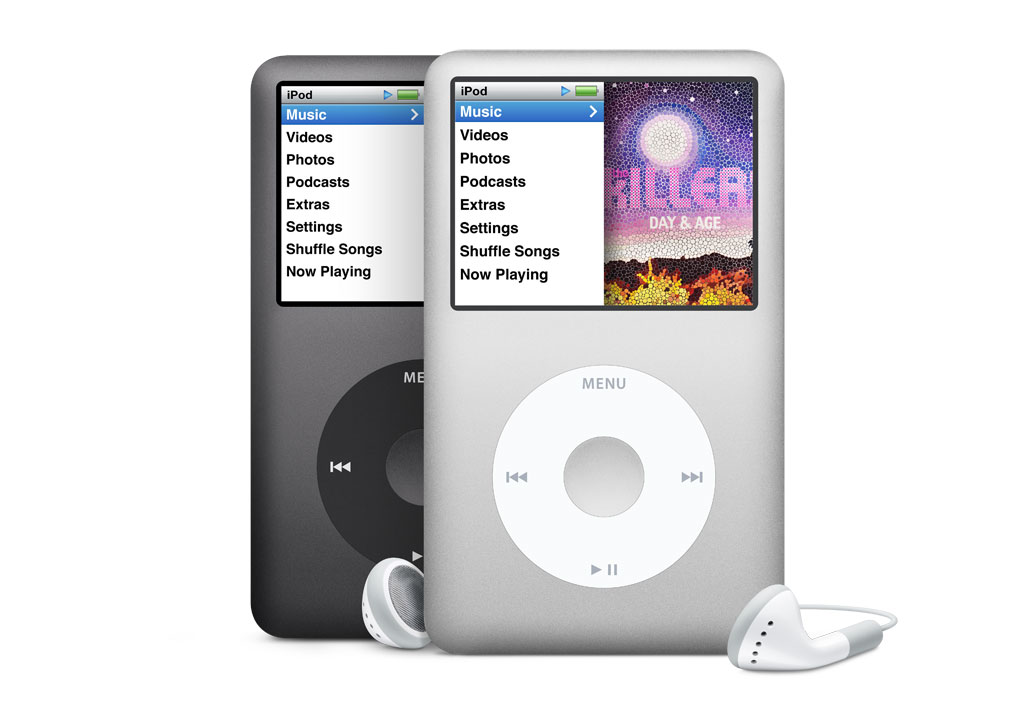
\includegraphics[height=14ex]{IPod.jpg}
		\end{column}
		\begin{column}{0.45\textwidth}
			Many highly successful consumer products were so because of their human-centred design focus. This
			is exemplified through \textit{Apple's iPod}.
		\end{column}
	\end{columns}
\end{frame}

\begin{frame}[fragile]{Socrative \texttt{JBYPC3BBY}}
    \textbf{List} examples of effective design in Apple's iPod.
\end{frame}

\begin{frame}{HCI and Interactive Systems}
	Interactive systems include more than just tech gadgets:
	
	\begin{itemize}
		\item Wristwatches
		\item Mobile phones
		\item Smart Televisions
		\item Microwave ovens
		\item etc.
	\end{itemize}
\end{frame}

\begin{frame}{Donald Norman's Refridgerator}
	In an ages gone, even refridgerators had design flaws (Norman, 2002, p. 14-15):
	
	\vspace{2ex}
			
	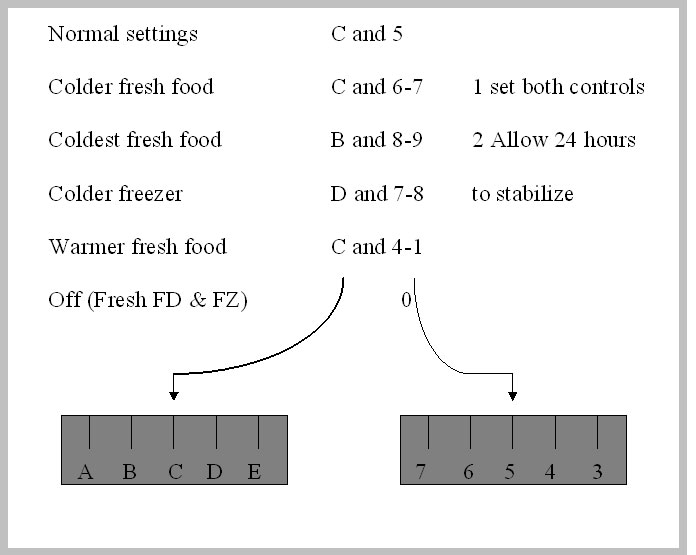
\includegraphics[height=24ex]{norman_fridge_controls.jpg}
\end{frame}

\begin{frame}{Donald Norman's Refridgerator}		
	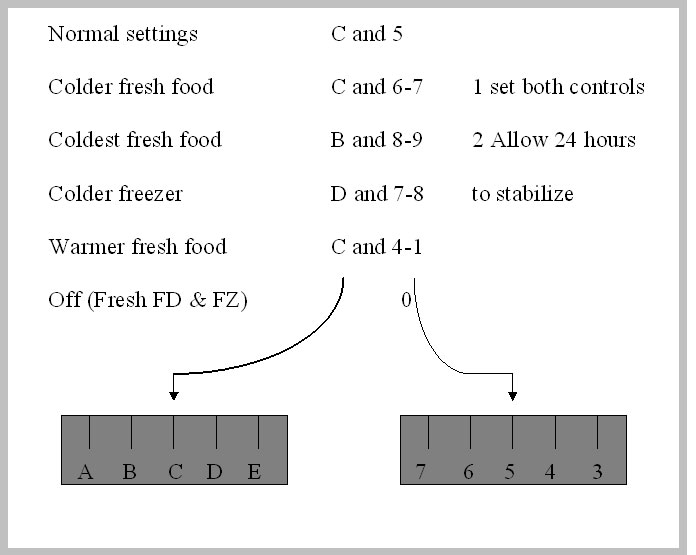
\includegraphics[height=24ex]{norman_fridge_controls.jpg}
	
	\vspace{2ex}
	
	\textbf{Illustrate} how you believe this fridge works. Post your diagram on Slack. You have 8 minutes.
\end{frame}

\begin{frame}{Donald Norman's Refridgerator}
	\begin{columns}[onlytextwidth]
		\begin{column}{0.45\textwidth}
			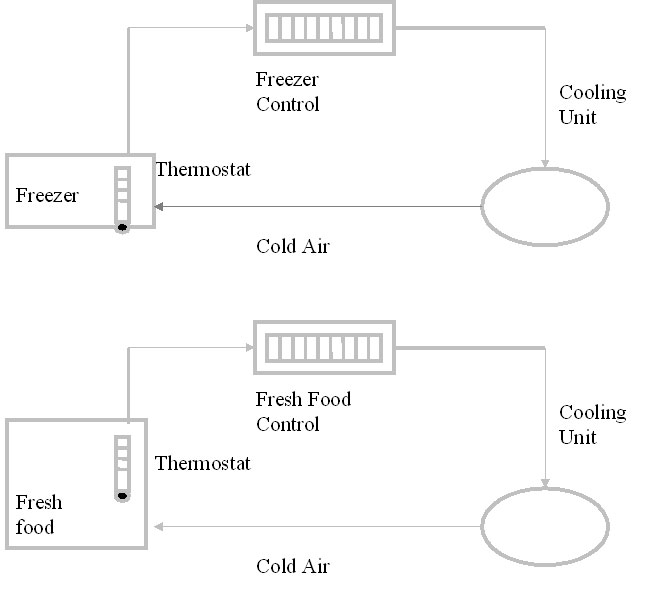
\includegraphics[height=20ex]{norman_fridge_mental_model.jpg}
			
			Option A
		\end{column}
		\begin{column}{0.45\textwidth}
			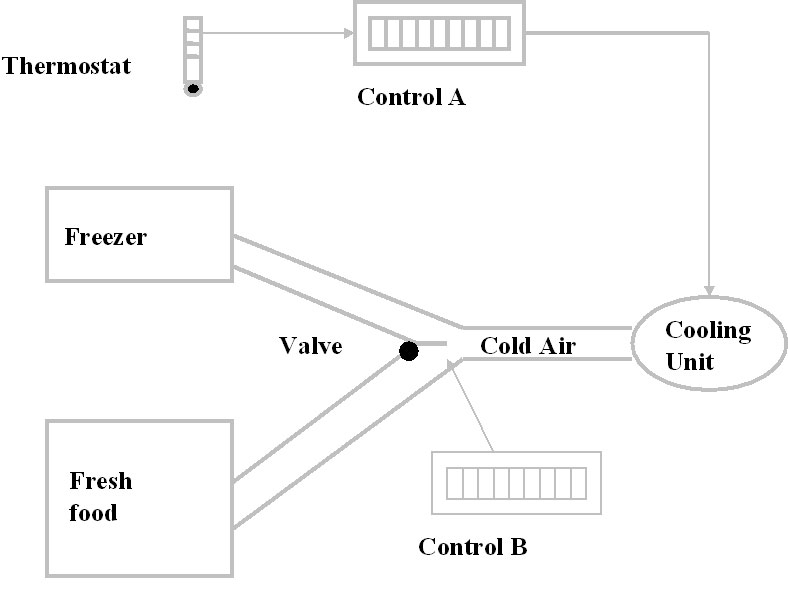
\includegraphics[height=20ex]{norman_fridge_actual_design.jpg}
			
			Option B
		\end{column}
	\end{columns}
\end{frame}

\begin{frame}{HCI and Interactive Systems}
	``Usability is a quality attribute that assesses how easy user interfaces are to use''.
	
	\vspace{2ex}
	
	(Neilsen, 2012)
\end{frame}

\begin{frame}[fragile]{Socrative \texttt{JBYPC3BBY}}
	\begin{itemize}
		\item A key concern of game designers, is of course, the usability of their design. 
		\item Discuss usability flaws in games with the person sitting next to you for 5-minutes.
		\item \textbf{List} examples for why usability is important in games.
	\end{itemize}
\end{frame}

\begin{frame}{HCI and Interactive Systems}
	Interaction is the key to understanding the role of HCI in designing usable user interfaces (and, thereby, successful games). 
	Such interaction assumes two forms of communication:
	
	\begin{itemize}
		\item Player to Game (i.e., pressing buttons, pointing the mouse, typing, etc.)
		\item Game to Player (i.e., displaying information, tactile feedback, etc.)
	\end{itemize}
\end{frame}

\begin{frame}[fragile]{Socrative \texttt{JBYPC3BBY}}
    \textbf{List} examples of player-to-game communication.
\end{frame}

\begin{frame}[fragile]{Socrative \texttt{JBYPC3BBY}}
    \textbf{List} examples of game-to-player communication.
\end{frame}

\begin{frame}{HCI and Interactive Systems}
	\begin{itemize}
		\item This two-way interaction is critical to the design and play of games.
		\item  It is what makes their design particularly challenging and interesting for computing professionals. 
		\item ...
	\end{itemize}
\end{frame}

\begin{frame}{HCI and Interactive Systems}
	\begin{itemize}
		\item As players of games, we have become engaged more and more with this two way process of providing
		the system with input, interpreting the output of the game, and responding accordingly with new input.
		\item This forms the \textbf{interaction cycle}.
		\item However, we need to take a step-back, as professionals, to be able to analyse the accordances of such a cycle.
	\end{itemize}
\end{frame}

\begin{frame}{So, What Is Human-Computer Interaction?}
	Human-computer interaction is the name of the approach we use to study and improve interactive systems. It is concerned with:
	
	\begin{itemize}
		\item The joint performance of tasks by humans and machines. 
		\item The structure of human-machine communication.
		\item Social and organisational interaction with machines.
		\item Human capabilities in machine use.
		\item ...
	\end{itemize}
\end{frame}

\begin{frame}{So, What Is Human-Computer Interaction?}
	Human-computer interaction is the name of the approach we use to study and improve interactive systems. It is concerned with:
	
	\begin{itemize}
		\item ...
		\item Interface mechanisms.
		\item Interface specification and implementation
		\item Design trade-offs.
		\item and many other concerns (see Dix, 1998 for further notes).
	\end{itemize}
\end{frame}

\begin{frame}{So, What Is Human-Computer Interaction?}
	\begin{itemize}
		\item It lies at the intersection between the social and cognitive sciences, on the one hand.
		\item and Computer Science and technology, on the other.
	\end{itemize}
\end{frame}

\begin{frame}{So, What Is Human-Computer Interaction?}
	The three main roles of HCI are:
	
	\begin{itemize}
		\item Analysing and designing specific interaction technologies (e.g. displays, pointing devices, user agents, etc.)
		\item Studying and improving the processes of technology development (e.g. usability quality assurance, design methods, evaluation techniques, etc.)
		\item Developing and evaluating new applications (e.g. multimedia, mulsemedia, other immersives, etc.)
	\end{itemize}
\end{frame}

\begin{frame}{So, What Is Human-Computer Interaction?}
	HCI integrates:
	
	\begin{itemize}
		\item Scientific research concerns... \pause
		\item ...with the engineering goal of improving usability of computers. \pause
		\item That is, improving the `fit' of games to their players --- and it is obviously easier to change the design of a game than it is to change its player.
		\item Or, to create both useful and usable computer systems.
	\end{itemize}
\end{frame}

\begin{frame}{So, What Is Human-Computer Interaction?}
	Interactive system designers (e.g. game designers) study and apply techniques from HCI in order to provide support for human activity:
	
	\begin{itemize}
		\item Making system use faster
		\item Less prone to error
		\item Require less learning or less explicit instruction
		\item Enable higher quality work
		\item Increase satisfaction
		\item and so on...
	\end{itemize}
\end{frame}

\begin{frame}{So, What Is Human-Computer Interaction?}
	\begin{itemize}
		\item This leads to a more principled approach to interactive system design that `fits' into the software engineering approaches
		\item This may follow \textbf{a formal methodology} or, as is the case for the game controller project, follow \textbf{a parallel approach}
		which loosely informs the software engineering
	\end{itemize}
\end{frame}

\begin{frame}{So, Who Are HCI Professionals?}
	There is a whole family of disciplines and job titles asspoated with HCI. Some examples include:

	\begin{columns}[onlytextwidth]
		\begin{column}{0.45\textwidth}
			\begin{itemize}
				\item Information Architect
				\item Usability Engineer
				\item User Experience Architect
				\item Web Designers
				\item Ergonomists
			\end{itemize}
		\end{column}
		\begin{column}{0.45\textwidth}
			\begin{itemize}
				\item Cognitive Engineers
				\item HCI Consultants
				\item User-Centred Designers
				\item GUI Designers
				\item Interface Engineers
			\end{itemize}
		\end{column}
	\end{columns}
\end{frame}

\begin{frame}[fragile]{Slack Discussion}
	\begin{itemize}
		\item \textbf{Who} contributes to HCI in games? 
		
		\vspace{2ex}
		
		\item Spend 10-minutes researching these role and post any interesting link between these disciplines and games development.
	\end{itemize}
\end{frame}

\begin{frame}{Designing for Usability in Games}
	\begin{itemize}
		\item The difficulty of designing good interactive systems lies in matching \textbf{usability} (i.e., the fit fo the system to its users) to their
		\textbf{functionlity} (i.e., the technical features of the interactive system.
		\item Although it is critical to consider `use' as an important feature of design, it is of equal, if not greater, importance to consider
		functionality. Games are \textit{supposed} to be challenging.
		\item We are, therefore, faced with a trade-off; something we will visit later because there are no right or wrong answers, only
		good or bad decisions in particular contexts.
	\end{itemize}
\end{frame}

\begin{frame}{Designing for Usability in Games}
	It is also important to consider the contributions of the various areas of HCI to effective user intefaces for games 
	(adapted from Preece \textit{et al}, 1994):

	\begin{itemize}
		\item \textbf{cognitive psychology}: understanding all forms of mental behaviour; used, for example, in the design of in-game menues,
		placement of components in the HUD, and sequencing of interface events (e.g. when issuing commands to soldiers in an RTS). It also provides
		methods for the study of interaction, such as experimental design, and the construction of (testable) cognitive models to predict activity in
		an interface. \pause
		
		\item ...
		
	\end{itemize}
\end{frame}

\begin{frame}{Designing for Usability in Games}
	It is also important to consider the contributions of the various areas of HCI to effective user intefaces for games 
	(adapted from Preece \textit{et al}, 1994):

	\begin{itemize}
		\item ...
		
		\item \textbf{social and organisational psychology}: understanding the nature and causes of human behaviour in social contexts, such as
		console parties, online multiplayer games, and economies of capital in virtual worlds; \pause
		
		\item \textbf{ergonomics and human factors}: matching human capabilities to their tools and designed environments; \pause
		
		\item \textbf{linguistics}: the study of language, used in the design of dialogue and dialogue options and in understand multiplayer communication; \pause
		
		\item ...
	\end{itemize}
\end{frame}

\begin{frame}{Designing for Usability in Games}
	It is also important to consider the contributions of the various areas of HCI to effective user intefaces for games 
	(adapted from Preece \textit{et al}, 1994):

	\begin{itemize}
		\item ...
		
		\item \textbf{sociology}: used in considering the implications of a particular design on society (e.g. dark patterns in app store rating systems); \pause
		
		\item \textbf{anthropology}: the interrealtionship and co-development of culture and technology; \pause
		
		\item \textbf{philosophy}: forming the theoretical underpinning of the sciences and social sciences; \pause
		
		\item \textbf{engineering and design}: in the sense of applied science and the actual practices used to develop games and game interfaces.
	\end{itemize}
\end{frame}

\begin{frame}[fragile]{Socrative \texttt{JBYPC3BBY}}
    \textbf{What} is Human-Computer Interaction?
\end{frame}

\begin{frame}[fragile]{Socrative \texttt{JBYPC3BBY}}
    \textbf{Why} is HCI relevant to games?
\end{frame}

%\part{Your first C++ program}
\frame{\partpage}

\begin{frame}
	\frametitle{Project setup}
	\begin{itemize}
		\item Open \textbf{Visual Studio 2015} from the Start menu
		\item Click \textbf{New Project}
		\item Choose \textbf{Templates $\to$ Visual~C++ $\to$ Win32 $\to$ Win32~Console~Application}
		\item Choose an appropriate name and location, and click \textbf{OK}
		\item Click \textbf{Finish}
		\item If asked about source control, click \textbf{Cancel}
	\end{itemize}
\end{frame}

\begin{frame}{Running it}
	\begin{itemize}
		\item Click X, or press \textbf{F5} \pause
		\item It worked, but the window disappeared before we could see it! \pause
		\item Solution 1: click \textbf{Debug $\to$ Start~Without~Debugging}, or press \textbf{Ctrl~+~F5}
		\item Solution 2: click in the left margin next to the \lstinline{return 0;} line to set a \textbf{breakpoint} ---
			a red circle should appear. Then click X.
	\end{itemize}
\end{frame}

%\part{Variables and types}
\frame{\partpage}

\begin{frame}[fragile]{Variables}
	\begin{columns}[onlytextwidth]
		\begin{column}{0.45\textwidth}
			In Python, variables exist the moment they are assigned to:
			\begin{lstlisting}[language=Python]
a = 10
b = 20
			\end{lstlisting}
			\pause
			Variables can hold values of any type:
			\begin{lstlisting}[language=Python]
a = 10
a = 3.14159
a = "Hello"
			\end{lstlisting}
		\end{column}
		\pause
		\begin{column}{0.45\textwidth}
			In C++, variables must be \textbf{declared} before use, and must be given a \textbf{type}:
			\begin{lstlisting}
int a = 10;
int b = 20;
			\end{lstlisting}
			\pause
			Variables can only hold values of the correct type:
			\begin{lstlisting}
int a = 10;
a = 17;      // OK
a = "Hello"; // Error
			\end{lstlisting}
		\end{column}
	\end{columns}
\end{frame}


% Move this to next week
%\part{Functions}
\frame{\partpage}

\begin{frame}[fragile]{Function definitions}
    \begin{itemize}
        \item We have already seen an example of a function definition
    \end{itemize}
    \begin{lstlisting}
int main()
{
    std::cout << "Hello, world!" << std::endl;
    return 0;
}
    \end{lstlisting}
    \begin{itemize}
        \item The function \lstinline{main} takes no parameters, and returns a value of type \lstinline{int}
    \end{itemize}
\end{frame}

\begin{frame}[fragile]{Function signatures}
    \begin{itemize}
        \item The \textbf{signature} of a function defines its return type, name, and parameters
    \end{itemize}
    \begin{lstlisting}
double foo(std::string x, int y, bool z)
    \end{lstlisting}
    \pause
    \begin{itemize}
        \item This function takes three parameters: \pause
        \lstinline{x} of type \lstinline{std::string}, \pause
        \lstinline{y} of type \lstinline{int}, \pause
        and \lstinline{z} of type \lstinline{bool} \pause
        \item It returns a value of type \lstinline{double}
    \end{itemize}
\end{frame}

\begin{frame}[fragile]{Functions without return values}
    \begin{itemize}
        \item It is possible to define a function which does not return a value, using the \lstinline{void} keyword
        in place of its return type
    \end{itemize}
    \pause
    \begin{lstlisting}
void printNumber(int n)
{
    std::cout << n << std::endl;
}
    \end{lstlisting}
\end{frame}

\begin{frame}[fragile]{Pass by value}
    \begin{itemize}
        \item Function parameters are passed \textbf{by value}:
        the function receives \textbf{copies} of the original variables
    \end{itemize}
    \pause
    \begin{lstlisting}
void changeName(std::string name)
{
    name = "Ed";
}

int main()
{
    std::string name = "Mike";
    std::cout << name << std::endl; // Mike
    changeName();
    std::cout << name << std::endl; // Mike
}
    \end{lstlisting}
\end{frame}

\begin{frame}[fragile]{Pass by reference}
    \begin{itemize}
        \item Parameters can be passed \textbf{by reference} using \lstinline{&}, allowing the function to modify them
    \end{itemize}
    \pause
    \begin{lstlisting}
void changeName(std::string& name)
{
    name = "Ed";
}

int main()
{
    std::string name = "Mike";
    std::cout << name << std::endl; // Mike
    changeName();
    std::cout << name << std::endl; // Ed
}
    \end{lstlisting}
\end{frame}

\begin{frame}[fragile]{One area where C++ is ``simpler'' than Python!}
    \begin{itemize}
        \item Recall from COMP110 week 6: in Python, basic data types (numbers, booleans, strings etc)
            are passed by value, and object types (lists, dictionaries, class instances) are passed by reference
        \pause
        \item In C++, everything is passed by value unless it is explicitly marked as a reference with \lstinline{&}
    \end{itemize}
\end{frame}

\begin{frame}[fragile]{Constant references}
    \begin{lstlisting}
void greet(std::string name)
{
    std::cout << "Hi " << name << std::endl;
}
    \end{lstlisting}
    \pause
    \begin{itemize}
        \item The string will be copied in order to be passed in \pause
        \item More efficient to pass a reference, and mark it \lstinline{const} to prevent accidental modification
    \end{itemize}
    \begin{lstlisting}
void greet(const std::string& name)
{
    std::cout << "Hi " << name << std::endl;
}
    \end{lstlisting}
    \pause
    \begin{itemize}
        \item (this is only worthwhile for large data structures like strings and vectors, not for basic data types)
    \end{itemize}
\end{frame}



\part{Practical Activity}
\frame{\partpage}

\begin{frame}{Practical Activity}
	\begin{itemize}
		\item \textbf{Read} the assignment brief on LearningSpace.
		\item \textbf{Identify} the game for which you intend to create a novel game controller for.
		\item \textbf{Visit} \url{falmouthgamesacademy.com/l1s1_2015.html} 
		and \textbf{download} some games to try out. You do not need to make your final choice today!
		\item \textbf{Analyse} the accordances of the game and its required forms of interaction.
		\item \textbf{Note} them down and \textbf{start prototyping} a control scheme using your \textit{Makey Makey} kit.
	\end{itemize}
\end{frame}

\begin{frame}{Coursework Progress}
	\begin{itemize}
		\item \textbf{Continue} the practical activity---develop a prototype.
		\item \textbf{Prepare} for the first sprint review to take place next week.
		\item \textbf{Write} the brief proposal in the \texttt{readme.md} file in the GitHub repository. 
		\item \textbf{Create} a set of user stories on the Trello Board. 
	\end{itemize}
\end{frame}

% -------------------------------------------------------

%\part{The compiler}
%\frame{\partpage}
%
%\begin{frame}
%	\frametitle{The build process}
%	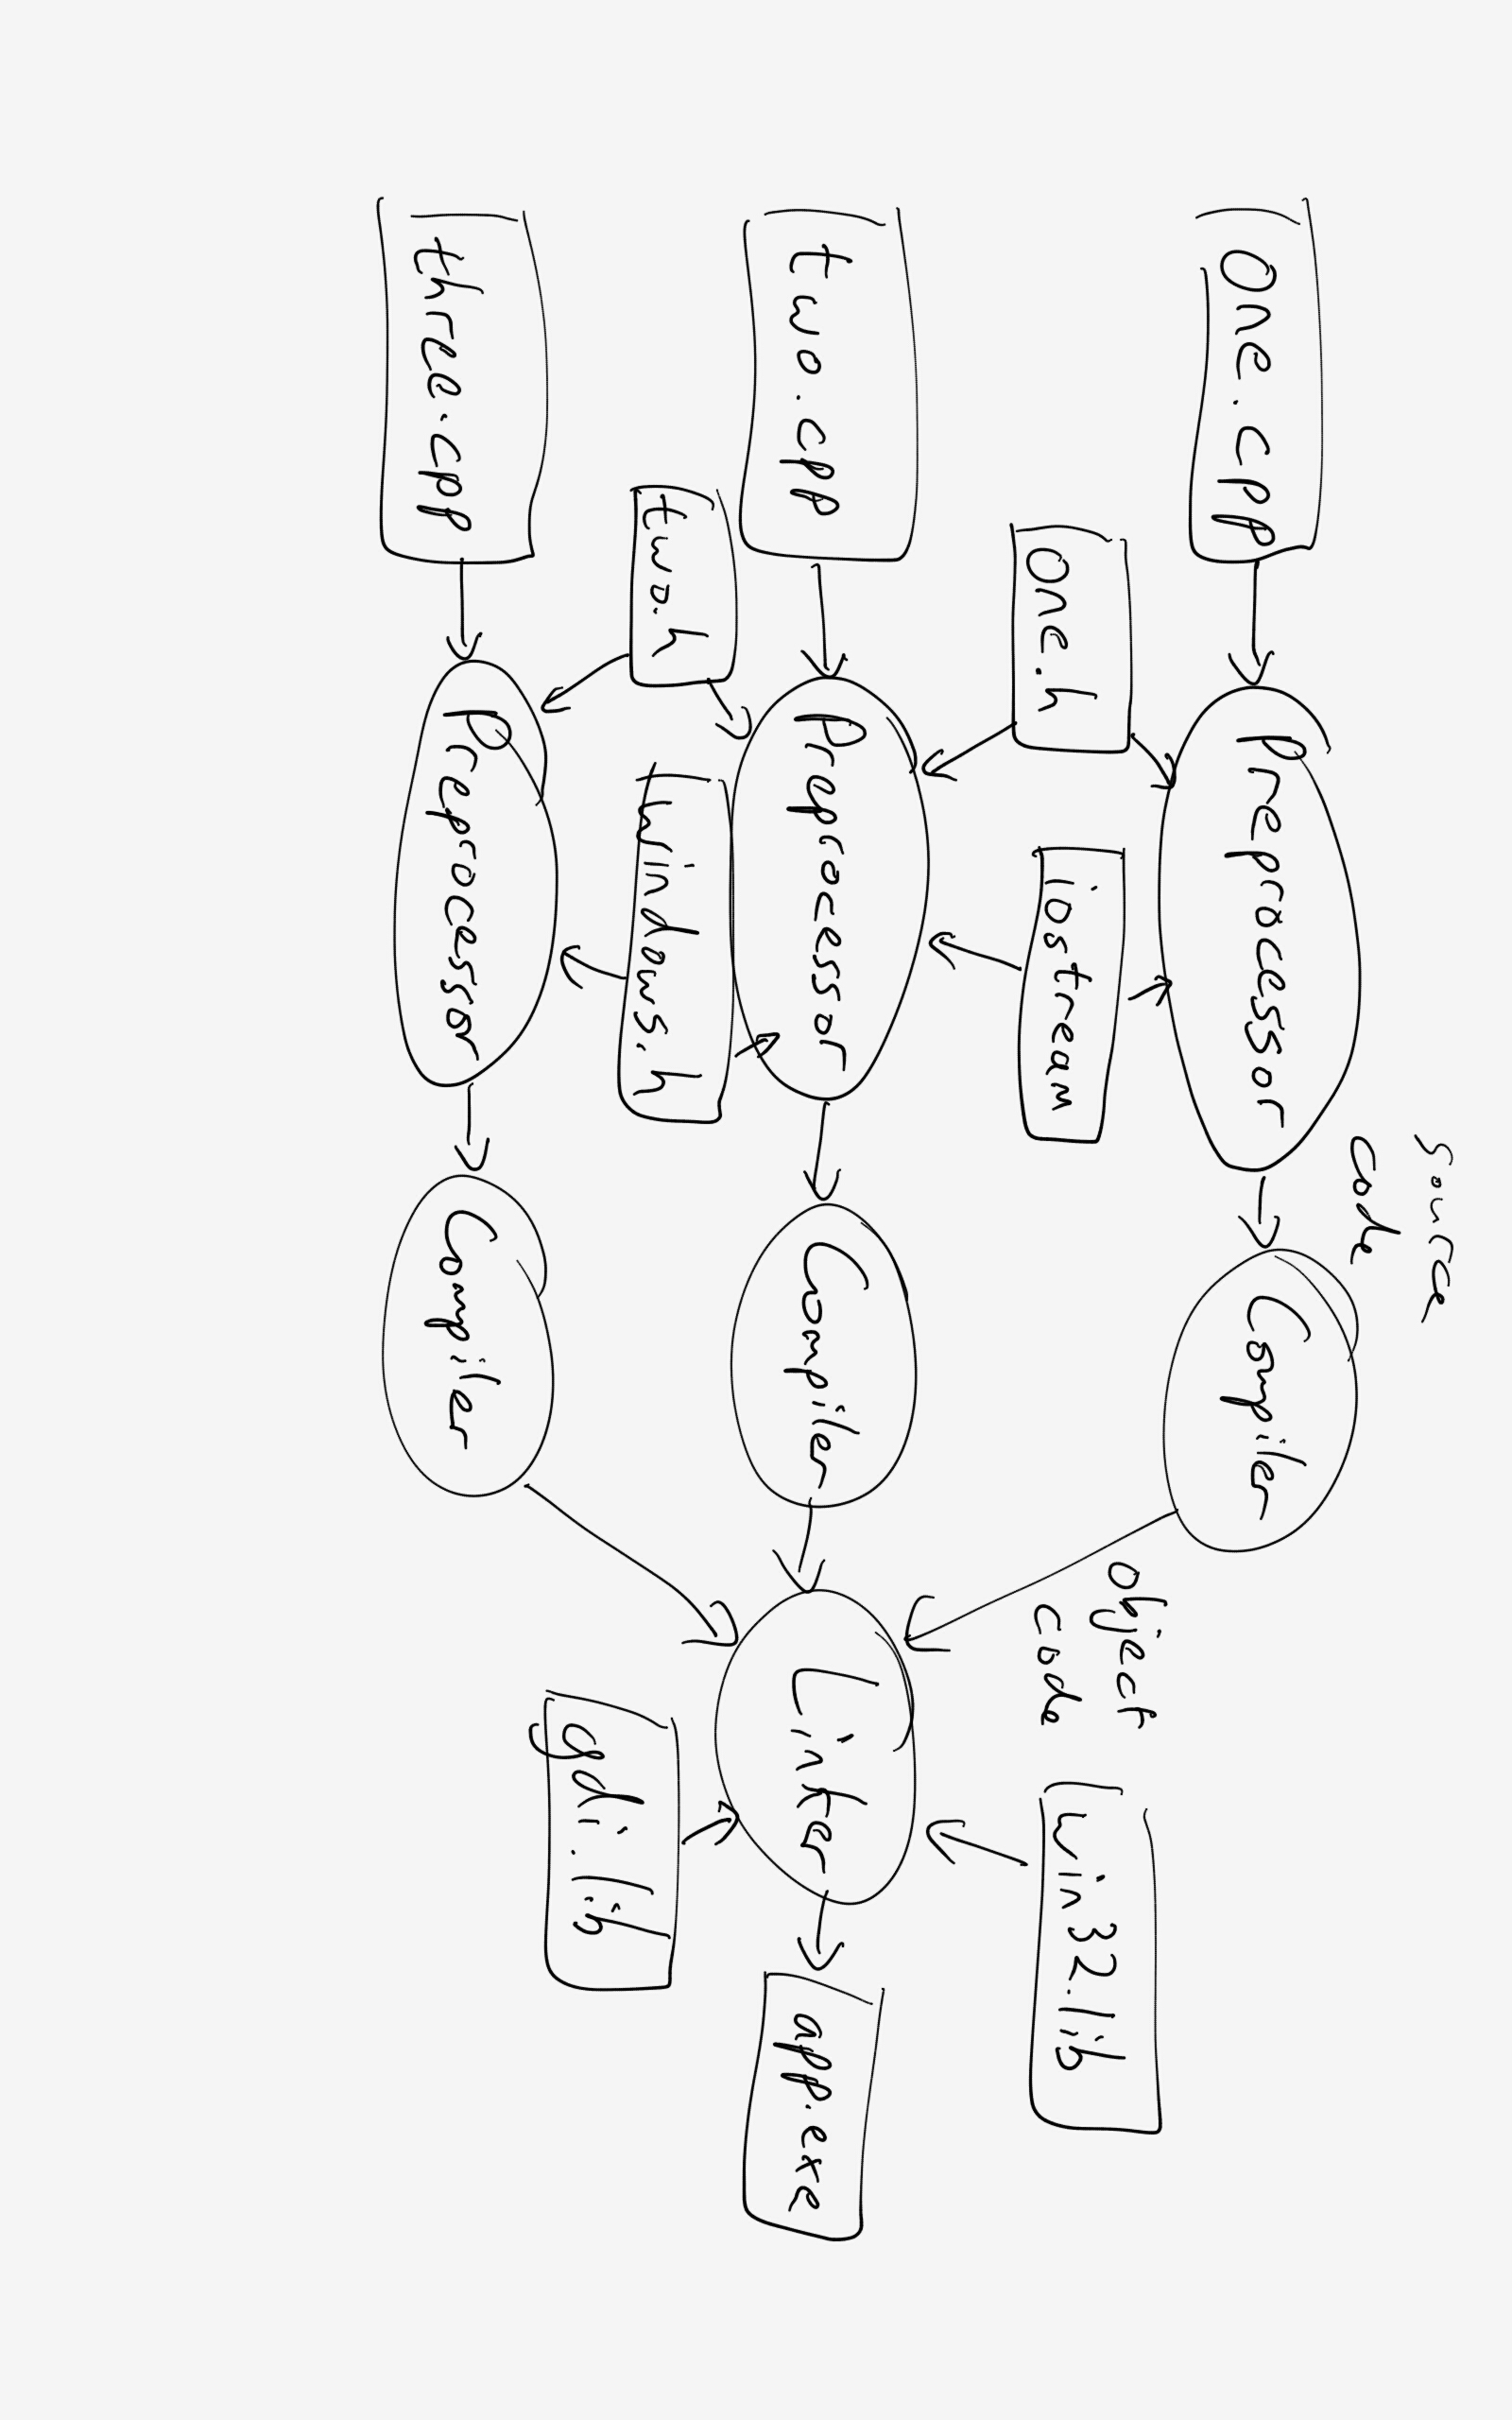
\includegraphics[height=\textwidth,angle=90]{compiler_sketch}
%\end{frame}

\end{document}
